\chapter{Color Spaces}
\label{ch:lesson18}

Previous chapters converted color images to grayscale and moved on. This chapter looks at what that conversion actually does, and at the other ways to represent color besides RGB, each suited to a different task: \textbf{HSV} (separating color from brightness), \textbf{YCbCr} (separating luminance from chrominance, the basis of video compression from Chapter~\ref{ch:lesson17}), and \textbf{L*a*b*} (designed so distances match human perception).

\section{Grayscale is already a color-space choice}

The simplest way to convert color to grayscale is to average the three channels, $Y=(R+G+B)/3$. The human visual system is actually more sensitive to green than to the other colors, so it's better to weight green more; a formula based on actual experiments on human subjects gives the weights used in \code{cv2.cvtColor(img, cv2.COLOR\_BGR2GRAY)}:
\begin{equation}
Y = 0.299R + 0.587G + 0.114B.
\end{equation}
These weights come from human luminance sensitivity: the eye is far more sensitive to green than to blue, so equal-intensity green and blue should \emph{not} map to the same gray level, even though a naive channel average would treat them identically. On pure green vs.\ pure blue patches: the naive average gives $85$ for both (indistinguishable), while the perceptually weighted version correctly reports green as much brighter ($150$) than blue ($29$) at the same channel intensity.

\subsection*{Why this formula is outdated (even though widely used, and still useful)}

Two things are hiding in that formula worth knowing about:
\begin{enumerate}
  \item \textbf{Old primaries.} The weights $0.299, 0.587, 0.114$ come from the 1953 NTSC standard (Rec.\ 601), derived from the specific red/green/blue phosphors used in early color CRT televisions. Modern LED displays use more saturated primaries, so the colorimetrically correct weights for a modern screen are actually $Y=0.2126R+0.7152G+0.0722B$ (Rec.\ 709/sRGB) --- noticeably \emph{more} green-weighted and \emph{less} red-weighted. \code{cv2.cvtColor} still uses the old Rec.\ 601 weights, mainly for backward compatibility with decades of existing code.
  \item \textbf{Assumes linear light.} The weighted-sum formula is only true luminance when $R,G,B$ are \emph{linear} light values. But stored pixel values are gamma-\emph{encoded}, not linear. \code{cv2.cvtColor} applies the weights directly to the raw encoded 8-bit values without decoding gamma first --- fast, and close enough for most computer-vision purposes, but not the physically correct luminance a display-calibration or photometry application would need. (To see the problem: a pure blue image, RGB $=(0,0,255)$, converts to a gray value of $29$ everywhere --- which will incorrectly appear almost completely dark, even though a fully saturated blue is a fairly bright color to the eye.)
\end{enumerate}

\section{RGB channels are highly correlated}

In most real images, lighting/shading variation dominates: a surface gets brighter or darker as a whole, scaling all three channels together. That means R, G, and B end up strongly correlated with each other --- not a very efficient or convenient way to separate ``what color is this'' from ``how brightly lit is this,'' as the scatter plot in Figure~\ref{fig:l18-1} shows.

\begin{figure}[h]
\centering
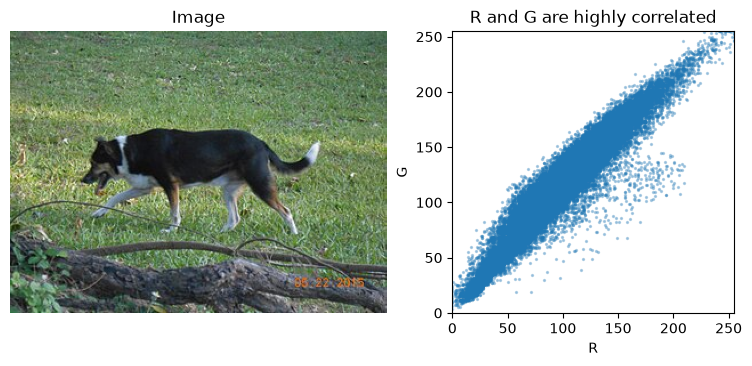
\includegraphics[width=0.85\textwidth]{figures/lesson18_fig01.png}
\caption{A real photo and a scatter plot of its R and G channel values --- tightly correlated (correlation coefficient $0.954$ on this image), because shading scales all three channels together.}
\label{fig:l18-1}
\end{figure}

\section{HSV: separating color from brightness}

HSV (Hue, Saturation, Value) reparametrizes color so that Hue captures \emph{which} color (independent of how bright or washed-out it is), Saturation captures how vivid/pure it is, and Value captures brightness alone. This makes color-based segmentation dramatically more robust to lighting than thresholding directly in RGB.

On a synthetic orange disk with a strong left-to-right lighting gradient: thresholding on HSV hue recovers the disk perfectly (IoU $1.000$ against the true disk), while a fixed RGB color range misses the darkened side entirely (IoU $0.710$), as Figure~\ref{fig:l18-2} shows.

\begin{figure}[h]
\centering
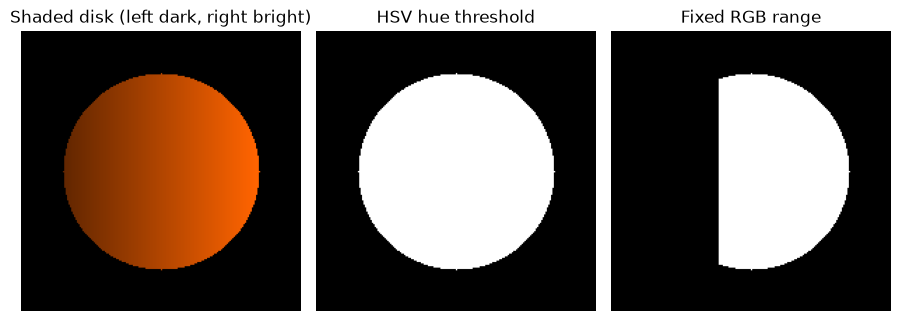
\includegraphics[width=0.9\textwidth]{figures/lesson18_fig02.png}
\caption{A shaded disk (dark on the left, bright on the right), an HSV hue threshold, and a fixed RGB range. Hue thresholding recovers the disk regardless of the lighting gradient; the RGB range misses the darkened side entirely.}
\label{fig:l18-2}
\end{figure}

\section{YCbCr: luma and chroma, and why video compresses color more aggressively}

YCbCr (used internally by JPEG and almost all video codecs) splits an image into \textbf{luma} ($Y$, roughly brightness) and two \textbf{chroma} channels ($C_b, C_r$, roughly ``how blue'' and ``how red''). The human visual system resolves fine spatial detail in luma far better than in chroma --- the biological basis for \textbf{chroma subsampling} (storing chroma at lower resolution than luma, e.g.\ video's common ``4:2:0'' format), one of the free compression wins used throughout Chapter~\ref{ch:lesson17}'s JPEG pipeline.

Subsampling either channel $8\times$ and measuring reconstruction error against the original: degrading chroma costs a mean absolute error of $6.44$ gray levels, while degrading luma by the same factor costs $10.15$ --- discarding the same amount of resolution costs noticeably less error in chroma than in luma, as Figure~\ref{fig:l18-3} shows.

\begin{figure}[h]
\centering
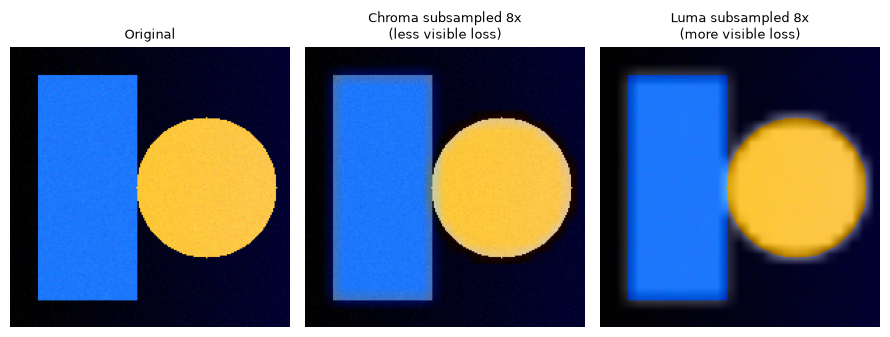
\includegraphics[width=0.9\textwidth]{figures/lesson18_fig03.png}
\caption{Original, chroma subsampled $8\times$ (barely visible loss), and luma subsampled $8\times$ (clearly visible loss) --- the same detail loss is simply less objectionable when it happens to color rather than brightness.}
\label{fig:l18-3}
\end{figure}

\section{L*a*b*: a perceptually uniform space}

RGB's Euclidean distance is a poor stand-in for how different two colors actually \emph{look}: equal RGB distances can correspond to wildly different perceived differences, depending on where in color space they fall. CIELAB was explicitly designed so that Euclidean distance between two L*a*b* colors approximates perceptual difference much more consistently --- useful for color-based quality metrics, clustering, and matching.

Generating 2000 random color pairs, each held at \emph{exactly} the same RGB distance ($30.0$): the resulting L*a*b* distances range from a minimum of $3.0$ to a maximum of $38.1$ (median $17.3$) --- more than a $12\times$ spread, depending purely on \emph{where} in color space the pair sits, as the histogram in Figure~\ref{fig:l18-4} shows.

\begin{figure}[h]
\centering
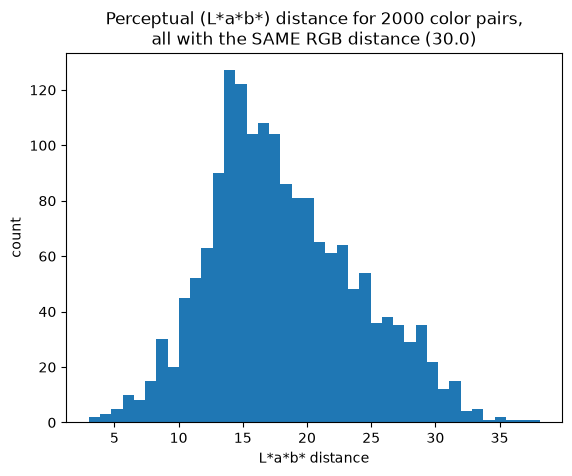
\includegraphics[width=0.55\textwidth]{figures/lesson18_fig04.png}
\caption{Histogram of L*a*b* distances for 2000 color pairs all held at the same RGB distance. Any algorithm using raw RGB distance as a proxy for perceptual similarity (nearest-neighbor color matching, k-means color clustering, background-subtraction thresholds) inherits this same distortion; switching to Lab distance is a simple, standard fix.}
\label{fig:l18-4}
\end{figure}

\subsection*{Exercises}
\begin{enumerate}
  \item Repeat the HSV vs.\ RGB segmentation demo with a shading gradient that also shifts hue slightly (e.g.\ blend toward a different color at one edge, not just changing brightness). Does hue-only thresholding still work as well?
  \item Increase the chroma/luma subsampling factor from 8 to 20. Does the qualitative story (chroma loss less visible than luma loss) still hold, or does it eventually break down?
  \item Find, by inspecting the color pairs in the Lab experiment, one example pair with a very \emph{small} Lab distance and one with a very \emph{large} L*a*b* distance (despite both having the same RGB distance). Display the four colors as swatches and describe, in your own words, why the low-Lab-distance pair looks more similar.
\end{enumerate}

\vfill
\fullcode{lesson18}{lesson18_color_spaces}
